
% part 12
\section{Сервер, преобразующий поэзию\label{sec:part12}}

\subsection{Еще один сервер}

Не смотря на то, что мы уже написали один Twisted сервер, давайте теперь 
напишем другой, и затем мы опять вернемся к изучению Deferred'в.


В главе 9 и 10 мы ознакомились с идеей движка, трансформирующего поэзию. 
Один из такик движков (cummingsifier) мы, в конечном итоге, реализовали, это 
было настолько просто, что нам пришлось добавить случайные исключения для 
эмуляции ошибки. Но, если бы трансформирующий движок был размещен на 
другом сервере, обеспечивая сетевой ``сервис, по трансформации поэзии'', то 
ошибка ``трансформирующий сервер не доступен'' была бы более реальной.  


Таким образом, в главе 12 мы собираемся реализовать 
поэтический трансформирующий сервер и, затем, в следующей главе, 
мы обновим наш поэтический клиент, для того, чтобы он 
мог использовать внешний трансформирующий сервис, и в процессе  
изучим несколько новых вещей по поводу Deferred'в.


\subsection{Проектирование протокола}


До сих пор взаимодействия между клиентом и сервером были строго 
одностороннее. Сервер отправляет поэму клиенту, в то время как 
клиент никогда вовсе ничего не отправляет серверу. Но, трансформирующий 
сервис является двунаправленным - клиент отправляет поэму серверу, 
затем сервер отправляет трансформированную поэму обратно.


Позволим серверу поддерживать несколько видов трансформаций и 
разрешим клиенту выбирать какой вид использовать. Клиент 
будет отправлять два куска информации: название трансформации и 
полный текст поэмы. Сервер будет возвращать один кусок информации, 
а именно: текст трансформированной поэмы. В итоге, мы получаем 
очень простую разновидность удаленного вызова процедур (\href{http://en.wikipedia.org/wiki/Remote\_procedure\_call}{Remote Procedure Call}). 


Twisted включает поддержку нескольких протокролов, 
которые мы могли бы использовать для решения этой 
проблемы, включая \href{http://twistedmatrix.com/trac/browser/tags/releases/twisted-8.2.0/twisted/web/xmlrpc.py}{XML-RPC}, \href{http://twistedmatrix.com/documents/current/core/howto/pb-intro.html}{Perspective Broker} и \href{http://twistedmatrix.com/trac/browser/tags/releases/twisted-8.2.0/twisted/protocols/amp.py}{AMP}. 


Но, включение любой из этих полнофункциональных протоколов 
увлекло бы нас вдаль, поэтому мы вместо этого будем использовать 
наш собственный скромный протокол. Давайте, клиент будет отправлять 
строку в форме (без угловых скобок):

\begin{scriptsize}\begin{verbatim}
<название преобразования>.<текст поэмы>
\end{verbatim}\end{scriptsize}


Это только название преобразования с последующей точкой и 
полным текстом поэмы. Все это мы будем кодировать в формате netstring. 
Сервер будет отправлять текст преобразованной поэмы, также в формате  
netstring. Поскольку netstring'и хранят длину строки, клиент 
сможет обнаружить случай, когда на стороне сервера возникает ошибка, 
в момент отправки результата (например, в середине операции сервер мог сломаться). 
Если вы вспомните, то наш изначальный поэтический протокол 
имел проблемы по обнаружению прерывания доставки поэзии.  


Возможно, что наш протокол не самый лучший, но его достаточно 
для цели изучения.

\subsection{Код}

Давайте посмотрим на код нашего трансформирующего сервера, 
расположенного в \href{http://github.com/jdavisp3/twisted-intro/blob/master/twisted-server-1/tranformedpoetry.py#L1}{twisted-server-1/tranformedpoetry.py}. Сначала мы определяем 
класс \href{http://github.com/jdavisp3/twisted-intro/blob/master/twisted-server-1/tranformedpoetry.py#L41}{TransformService}:

\begin{scriptsize}\begin{verbatim}
class TransformService(object):

    def cummingsify(self, poem):
        return poem.lower()
\end{verbatim}\end{scriptsize}


Трансформирующий сервис на данный момент поддерживает 
только одну трансформацию - cummingsify, через метод 
с тем же названием. Мы могли бы добавить дополнительные алгоритмы 
используя дополнительные методы. Тут важно отметить следующее: 
трансформирующий сервис полностью независим от определенных 
деталей протокола, про который мы договорились ранее. Отделение логики 
протокола от логики сервиса - это общий шаблон программирования  
в Twisted. Использование этого шаблона позволяет без дублирования кода 
предоставлять один и тот же сервис через различные протоколы.


Теперь давайте посмотрим на 
\href{http://github.com/jdavisp3/twisted-intro/blob/master/twisted-server-1/tranformedpoetry.py#L67}{protocol factory} (мы будем смотреть на протокол после):

\begin{scriptsize}\begin{verbatim}
class TransformFactory(ServerFactory):

    protocol = TransformProtocol

    def __init__(self, service):
        self.service = service

    def transform(self, xform_name, poem):
        thunk = getattr(self, 'xform_%s' % (xform_name,), None)

        if thunk is None: # no such transform
            return None

        try:
            return thunk(poem)
        except:
            return None # transform failed

    def xform_cummingsify(self, poem):
        return self.service.cummingsify(poem)
\end{verbatim}\end{scriptsize}


Данная factory предоставляет метод transform, который 
может использоваться экземпляром protocol для запроса 
трансформации поэзии на стороне присоединенного клиента. 
Метод возвращает None, если не существует запрашиваемой 
трансформации или, если преобразование не выполнилось. И, 
подобно TransformService, protocol factory независит от 
типа сетевого протокола, детали которого реализуются в самом 
классе protocol. 


Одно замечание: мы защищаем доступ до сервиса через 
методы, имеющие префикс xform\_. Это шаблон, который 
вы найдете в исходниках Twisted, хотя префиксы 
варьируются. Это один из способов предотвратить 
клиентский код от выполнения произвольного метода 
над сервисным объектом, поскольку клиент может отправить 
любое название трансформации. Также это является 
местом для выполнения протокольно-специфичной адаптации к 
API, предоставленную сервисным объектом. 


Теперь мы посмотрим на 
\href{http://github.com/jdavisp3/twisted-intro/blob/master/twisted-server-1/tranformedpoetry.py#L47}{реализацию протокола}:

\begin{scriptsize}\begin{verbatim}
class TransformProtocol(NetstringReceiver):

    def stringReceived(self, request):
        if '.' not in request: # bad request
            self.transport.loseConnection()
            return

        xform_name, poem = request.split('.', 1)

        self.xformRequestReceived(xform_name, poem)

    def xformRequestReceived(self, xform_name, poem):
        new_poem = self.factory.transform(xform_name, poem)

        if new_poem is not None:
            self.sendString(new_poem)

        self.transport.loseConnection()
\end{verbatim}\end{scriptsize}

%In the protocol implementation we take advantage of the fact that Twisted supports netstrings via the NetstringReceiver protocol. That base class takes care of decoding (and encoding) the netstrings and all we have to do is implement the stringReceived method. In other words, stringReceived is called with the content of a netstring sent by the client, without the extra bytes added by the netstring encoding. The base class also takes care of buffering the incoming bytes until we have enough to decode a complete string.

В реализации протокола мы воспользуемся тем 
фактом, что Twisted поддерживает netstring'и в 
реализации протокола 
\href{http://twistedmatrix.com/trac/browser/tags/releases/twisted-8.2.0/twisted/protocols/basic.py#L31}{NetstringReceiver}. Этот  
базовый класс кодирует и декодирует netstring'и, и 
все, что мы должны реализовать, - метод 
\href{http://twistedmatrix.com/trac/browser/tags/releases/twisted-8.2.0/twisted/protocols/basic.py#L49}{stringReceived}. 
Метод stringReceived вызывается с содержимым 
netstring'а, отправленым клиентом, без дополнительных 
байт, добавляемых при кодировании строки в netstring (без заголовка). 
Базовый класс NetstringReceiver также заботится о буферизации входящих 
байт до тех пор пока у нас не будет достаточно для декодирования.


Если все прошло хорошо (и если мы не закрыли соединение), 
мы отправляем трансформированную поэму обратно клиенту, 
используя метод sendString, предоставляемый 
NetstringReceiver (и который в итоге вызывает transport.write()). 
Мы не будем больше надоедать функцией 
\href{http://github.com/jdavisp3/twisted-intro/blob/master/twisted-server-1/tranformedpoetry.py#L89}{main}, поскольку она подобна рассмотренным ранее.


Заметьте, что мы продолжаем
Twisted шаблон, переводящий входный 
поток байт, к более и более высоким 
уровням абстракции путем определения метода 
xformRequestReceived, который вызывается с двумя независимыми 
аргументами: название трансформации и сама поэма.


\subsection{Простой клиент}


Мы реализуем Twisted клиент для преобразующего 
сервиса в следующей части, а на данный момент мы 
просто обойдемся простым скриптом, расположенным в twisted-server-1/transform-test.
В скрипте используется программа netcat, 
которая отправляет поэму серверу и печатает его ответ (который 
будет кодирован как netstring). Допустим, что вы запустили 
трансформирующий сервер на порту $11000$:

\begin{scriptsize}\begin{verbatim}
python twisted-server-1/tranformedpoetry.py --port 11000
\end{verbatim}\end{scriptsize}

Тестирующий скрипт можно запустить так:

\begin{scriptsize}\begin{verbatim}
./twisted-server-1/transform-test 11000
\end{verbatim}\end{scriptsize}

И вы увидите примерно следующее:

\begin{scriptsize}\begin{verbatim}
15:here is my poem,
\end{verbatim}\end{scriptsize}

Это трансформированная поэма в виде netstring (оригинальная в верхнем регистре).


\subsection{Обсуждение}


В этого главе мы ознакомились с несколькими новыми идеями:

\begin{enumerate}
\item Двунаправленной коммуникацией
\item Встраивание протокола, реализованного в Twisted
\item Использование сервисного объекта для разделения функциональной и 
протокольной логики
\end{enumerate} 


Основные механизмы двунаправленной коммуникации простые. 
Мы использовали те же самые приемы для чтения и 
записи данных в предыдущих клиентах и серверах; 
единственное отличие в том, что мы их использовали вместе. 
Конечно же, более сложный протокол потребует более 
сложного кода для обработки байтового потока и 
форматирования выходных сообщений. И есть огромная причина 
использовать существующую реализацию протокола подобно тому, 
как мы это сделали сегодня.


Как только вам становится комфортно писать базовые протоколы, 
хорошая идея - посмотреть на различные реализации протоколов в Twisted. 
Вы можете начать с просмотра 
\href{http://twistedmatrix.com/trac/browser/tags/releases/twisted-8.2.0/twisted/protocols/basic.py}{twisted.protocols.basic} модуля и продолжить оттуда. Написание 
простых протоколов - это прекрасный способ познакомить 
себя со стилем программирования в Twisted, но в 
<<реальной>> программе, вероятнее, что более общим 
является использование готовой реализации, предполагая, что 
она есть.
 

Последняя идея, с которой мы познакомились, - использование 
объекта Service для разделения функциональной и протокольной 
логики, является действительно выжным шаблоном проектирования 
с использованием Twisted. Хотя, сервисный 
объект, который мы сегодня сделали является тривиальным, 
вы можете представить более реалистичный сетевой сервис, 
который мог бы быть достаточно сложным. Создавая Service независимым от
деталей протокола, мы можем быстро предоставить тот же самый сервис 
по новому протоколу без дублирования кода.


Рисунок \ref{fig:server-21} показывает трансформирующий сервер, 
предоставляющий трансформацию поэзии через два различных 
протокола (версия сервера, который мы представили выше предоставляет 
только один протокол):

\begin{figure}[h]
\begin{center}
    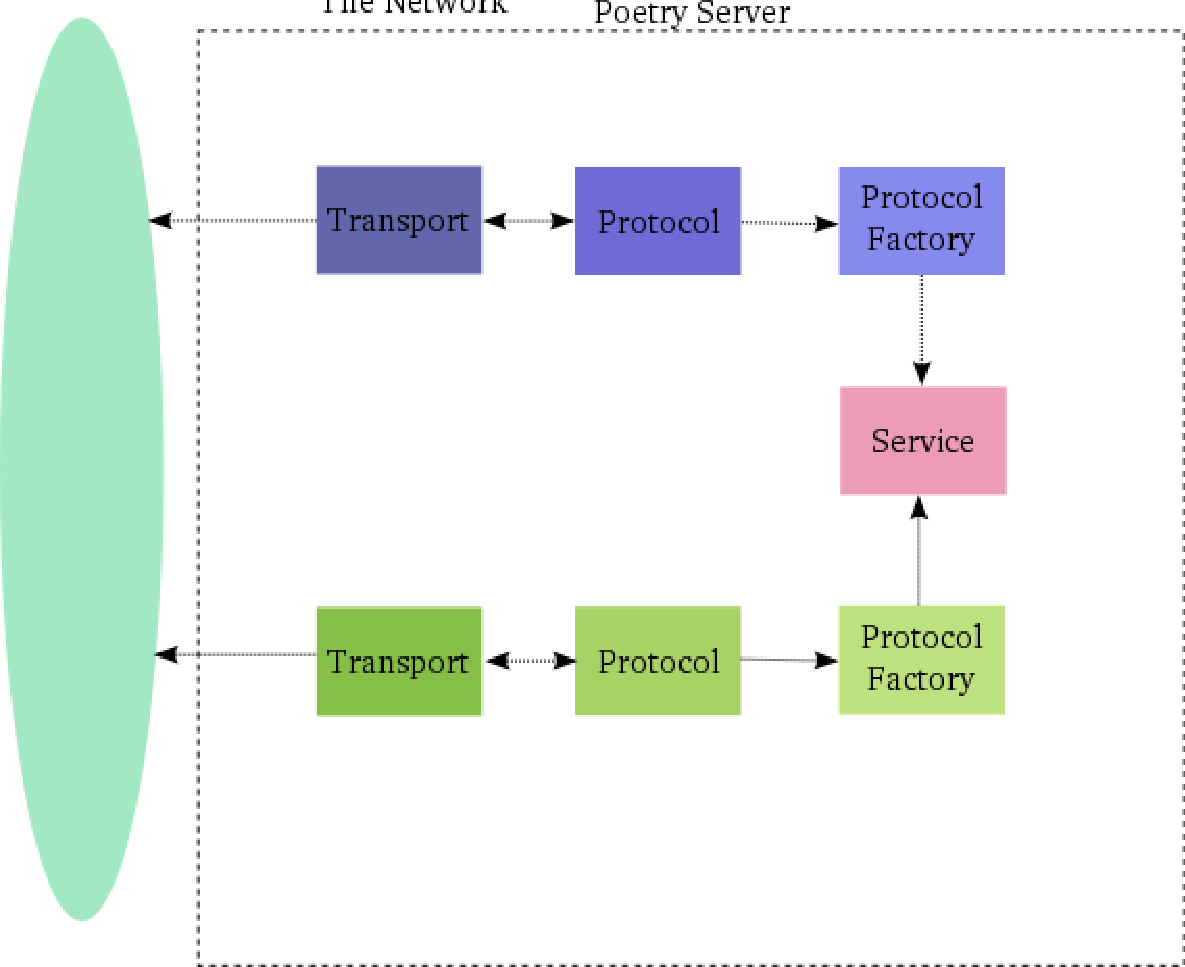
\includegraphics[width=0.8\textwidth]{images/server-21.pdf}
    \caption{Трансформирующий сервер с двумя протоколами\label{fig:server-21}}
\end{center}
\end{figure}

Хотя нам нужно две различных protocol factory, как это 
изображено на рисунке \ref{fig:server-21}, они могли бы отличаться 
только их классовым атрибутом protocol и были в остальном 
идентичными. Фабрики (factory) могли бы  
разделять один и тот же объект Service, и только сами Protocol требовали 
бы разной релизации.


\subsection{Взгляд в будущее}


В главе 13, мы обновим наш поэтический клиент так, чтобы он мог использовать 
трансформирующий сервер вместо реализации трансформаций в самом 
клиенте. 

\subsection{Упражнения}

\begin{enumerate}

\item Прочитайте исходный код для класса NetstringReceiver. Что 
произойдет, есди клиент отправит неправильный netstring? Что 
случится, если клиент попытается отправить огромный netstring?

\item Изобретите другой трансформирующий алгоритм и добавьте его в 
трансформирующий сервис и protocol factory. Протестируйте его, поменяв 
netcat клиент

\item Изобретите другой протокол для запрашивания поэтических 
трансформаций и поменяйте сервер так, чтобы он мог управлять 
обоими версиями протоколов (на различных портах). Используйте 
тот же экземпляр TransformService для обоих.

\item Как нужно было бы поменять код, если методы 
для TransformService были бы асинхронные (например, они возращали бы Deferred'ы)? 

\item Напишите синхронный клиент для трансформирующего сервера.

\item Обновите изначальный клиент и сервер так, чтобы они использовали 
netstring'и при посылке поэзии. 

\end{enumerate}

